\chapter{Introduction}

\begin{enumerate}
    \item Motivation \& Relevance
    \item Domain and Motivation: e.g. \ac{SAR}, semantic Navigation, exploration in unknown environments, etc.
    \item Which solutions exist? Comparison of general properties and performance metrics:
    \begin{enumerate}
        \item \ac{OneMap} \cite{busch2025onemap}
        \item \ac{VLMaps} \cite{huang23vlmaps}
        \item \ac{VLFM} \cite{yokoyama2024vlfm}
        \item \ac{ConceptGraphs} \cite{gu2023conceptgraphsopenvocabulary3dscene}
        \item \ac{SemExp} \cite{chaplot2020semexp}
        \item \ac{GeFF} \cite{qui2024geff}
    \end{enumerate}

    \begin{figure}[h!]
    \centering
    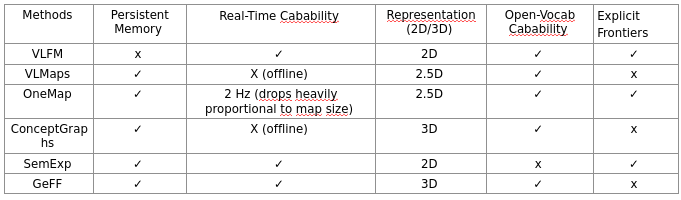
\includegraphics[width=\textwidth]{Images/1_introduction/temp_sota_comparison_common_properties.png}
    \caption{Comparison of state-of-the-art methods regarding common properties.}
    \label{fig:sota_comparison}
    \end{figure}

    \begin{figure}[h!]
    \centering
    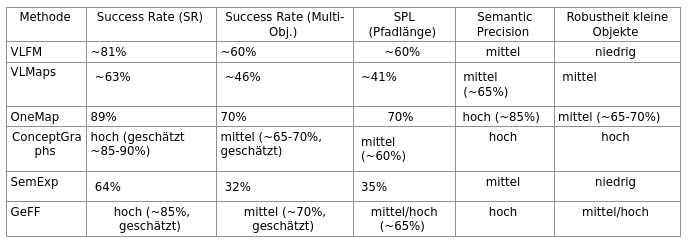
\includegraphics[width=\textwidth]{Images/1_introduction/temp_sota_comparison_performance_metrics.png}
    \caption{Comparison of state-of-the-art methods regarding performance metrics.}
    \label{fig:sota_performance}
    \end{figure}

    \item What is the technical problem? A combination of the following:
    \begin{enumerate}
        \item No persistent memory
        \item Not Real-Time
        \item 3D-Representation
        \item Sensibility to false positives for zero shot object detection
    \end{enumerate}
    \item Scientific Contribution:
    \begin{itemize}
        \item Development of a hybrid semantic exploration framework that combines \ac{VLFM}-based \cite{yokoyama2024vlfm} frontier scoring with Open-Fusion's \cite{kashu2023openfusion} global 3D scene representation, enabling multi-object search with open-vocabulary queries (text\sout{, image, audio}) during autonomous exploration. The approach is evaluated for improvements in overall and multi-object success rate (\ac{SR}) as well as path efficiency measured by success weighted by path length (\ac{SPL}).
        \item Implementation of a lightweight \ac{VLFM} \cite{yokoyama2024vlfm} component leveraging \ac{SEEM} \cite{zou2023seem} as a unified vision-language model, substantially reducing GPU memory requirements compared to traditional \ac{VLFM} \cite{yokoyama2024vlfm} pipelines using multiple separate models.
        \item Design of a sensor-based fusion strategy that integrates semantic detections from \ac{SEEM} \cite{zou2023seem} with clustered relevance fields from Open-Fusion \cite{kashu2023openfusion}, applying spatial confidence weighting to enhance robustness against false positives in zero-shot object detection.
        \item Experimental validation of the proposed system on a real mobile robot, focusing on practical aspects such as real-time performance and robustness to sensor noise including depth inaccuracies and changing lighting conditions.
    \end{itemize}

    \item Structure of the thesis:
\end{enumerate}
